\section{Technique}

The main objectives of the proposed visualization were:

\begin{enumerate}
\item to give a macro panoramic macro view of the evolution of EC number annotations
\item to allow users to explore the complete set of changes formulating and answering general questions about EC number changes
\end{enumerate}

Concerning the first objective, we would like to present at once all the changes segmented by all the possible combinations of events considering the three parameters of the model (common prefix length and number of generalizations and specializations) across all the database releases.

\subsection{Multivariate display}

We have a multivariate problem where the fundamental activity is to compare multiple instances of several variables at once and to allow users to identify similarities and differences among them. Small multiples of Tufte  \cite{tufte_envisioning} or trellis displays \cite{cleveland_trellis1,cleveland_trellis2}, as proposed by Cleveland, are a straightforward approach to present our data. They consists of splitting the data into multiple graphs that are presented at the same time in close proximity in the screen and allows to examine data in any one grahh more easily, and comparison of values and patterns among graphs with relative ease. 
According to Few \cite{few_nysi}, individual graphs display a subset of a data set divided according to a categorical variable and the several graphs differ only in terms of data. Every graph is the same type, shape, size and shares the same categorical and quantitative scales. Scales in each graph must start and end with the same values (otherwise the accurate comparison is more difficult). Graphs can be arranged horizontally or vertically or as a matrix in a meaninful order. 

Having this in mind, we proceed explaining the proposed visual representation. The basic graph of the proposed small multiple representation, which we call from now on \textit{frame}, is presented in Figure \ref{fig:technique}. It is a 2D plot where we present in x-axis the number of generalizations and in the y-axis, the number of generalizations. 
Both x and y-axes varies in the interval [0,4]. Position (0,0) from frames represents entries with no changes in the corresponding pair of versions. It is important to point out that there are prohibited positions for some lengths of common prefixes. For instance, if a change keeps a common prefix of size 3, it is impossible to have 2 generalizations. They are presented in a darked shade of gray in Figure \ref{fig:technique}.

\begin{figure}[htb]
  \centering
  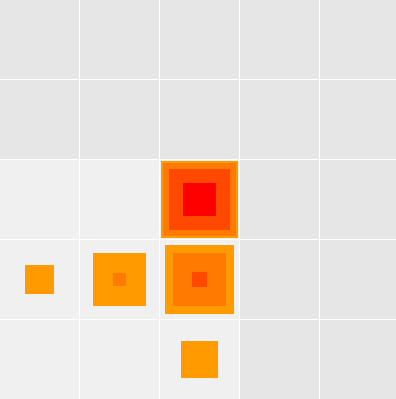
\includegraphics[width=3.5cm]{images/techniquea.png} (a) 
  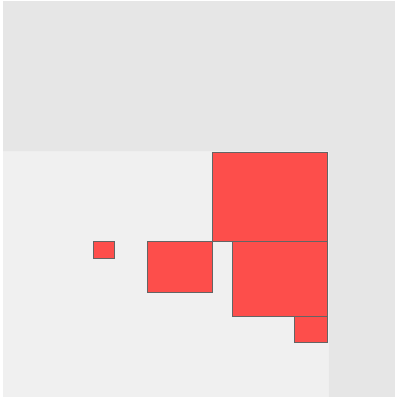
\includegraphics[width=3.53cm]{images/techniqueb.png} (b)
  \caption{Basic frames for the proposed small multiple visualization. In (a), we present the heatmap version and in (b), the squaremap. \textcolor{red}{Mudar para vers\~ao com heatmap de uma cor e com legendas}}
  \label{fig:technique}
\end{figure}

Several frames like this are then arranged in a small multiple fashion as in Figure \ref{fig:heatmap000}. In x-axis, we represent the consecutive pairs of released versions. The y-axis presents the possible common prefixes in [0,4]. 

\begin{figure*}[htb]
  \centering
  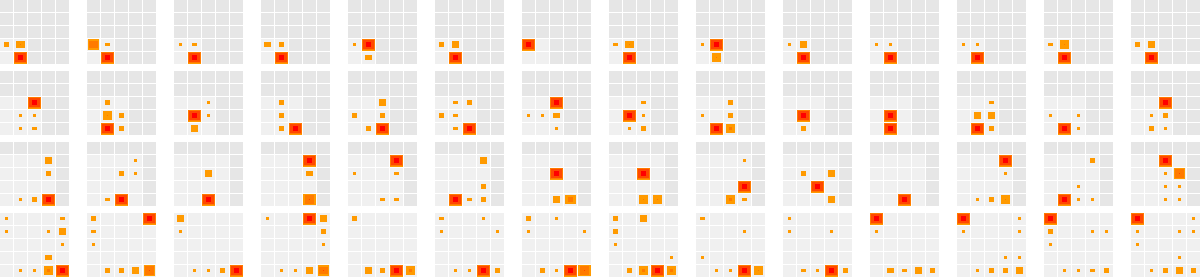
\includegraphics[width=17cm]{images/heatmap000.png}
  \caption{Multivariate view with heatmaps. \textcolor{red}{Mudar para vers\~ao com heatmap de uma cor e com legendas}}
  \label{fig:heatmap000}
\end{figure*}

\subsubsection{Heatmap}
\label{heatmap}

In a first version of the graph, we use a heatmap representation where color is a pre-attentive attribute that encodes the frequency of that configuration of change.

This representation aimed at giving an overview of the complete data evidencing trends and exceptions across the 15 releases. An interesting feature of this representation is that values in the lower right triangular matrix represents specialization and in the upper left triangular matrix, generalizations. Consequently, it is easy to recognize global trends towards generalization or specialization patterns in enzyme reaction annotations.

\subsubsection{Squaremap}
\label{squaremap}

Heatmaps present important trends in terms of generalization and specialization occurences however we see two possible drawbacks in that approach. 

Firstly, color is not a pre-attentive \textcolor{red}{???} which can preciselly encode quantitative data. For sure, one can perceive that a intense color represent a higher value than a less intense one. Hoever, it is very difficult to estimate preciselly the quantitative values from color intensities. 

The second drawback is that our heatmap presents two much blank space. According to Tufte \cite{tufte_envisioning}, the data density of a graph is the proportion of the total size of the graph that is dedicated displaying data. Tufte prefers high data density graphs as the human perceptual system is capable of detecting subtile patterns, trends and exceptions. On account of that, we decided to propose a second complementary view trying to reduce blank (non-data) space and also a representation which should use a more precise visual attribute to enconde the frequencies. 

The Squaremap representation was inspired in 2D scatterplots where the points are squares whose area represent frequency. Even though area is not the most precise visual attribute to enconde quantity, one can estimate its area through square side length which users can preciselly represent quantitative data. Notice, in Figure \ref{fig:technique}, that is easier to estimate quantities in the Squaremap (b) tnan in the Heatmap (a).

\subsection{Analytical interaction and navigation}

\subsubsection{Filtering, scales and normalization options}

The effective of the information visualization techniques hinge on the ability to clearly and accurately represent information and on the ability to interact with it to figure out what information means. Indeed, no matter how rich the display is, it will invite questions and the interaction is necessary to pursue an answer. Besides, different perspectives can lead to different insights. The proposed visualization allows pre-defined filters and different scalling and normalization options: 

\begin{enumerate}
\item log scale on the frequencies
\item normalization of frequencies by frame or globally
\item filter by only changes (removing position (0,0)) or presentation of the complete data set
\end{enumerate}

\subsubsection{Micro/macro view}

One particularly interesting way to create dense graphics is through what Tufte calls micro/macro readings \cite{tufte_envisioning}. These graphics convey one layer of information on a micro scale and another layer on a zoomed out, macro scale. One nice consequence of this technique is information is consumed hierarchically. The viewer may glance from a distance to observe an aggregate trend, and later peer in closely to examine individual pieces of that trend. Our multivariate view is a macro view of the whole changes data set. Users can click each frame and see it zoomed in a micro view. 

\subsubsection{Exploratory navigation}

Besides having a micro/macro view of the possible changes in enzyme annotation, users can click the points in the micro view and see interactive histograms of each type of change. Through these histograms users can see the enzyme families which has suffered that change. These histograms are composed by small squares representing each change and by clicking individual points users can see details about the entry. 

%\begin{figure*}[htb]
%  \centering
%  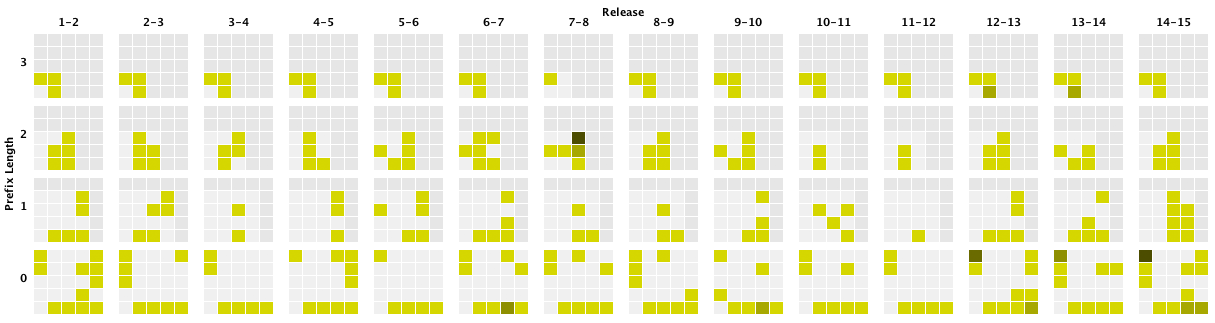
\includegraphics[width=17cm]{images/heatmap001.png}
%  \caption{Heatmap, only changes, no log scale, global normalization}
%\end{figure*}

%\begin{figure*}[htb]
%  \centering
%  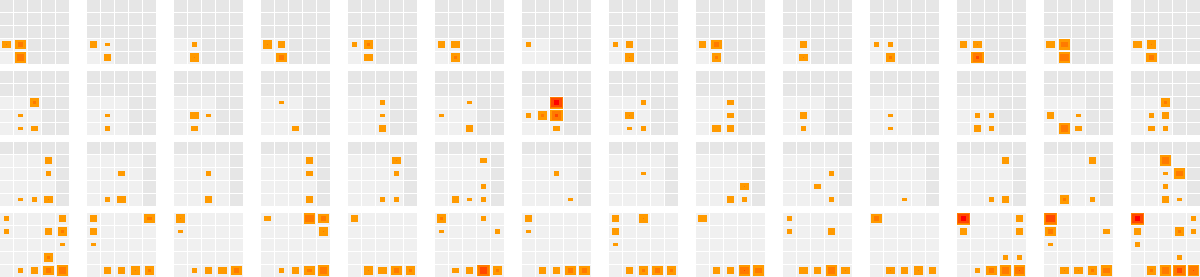
\includegraphics[width=17cm]{images/heatmap101.png}
%  \caption{Heatmap, only changes, log scale, global normalization}
%\end{figure*}

%\begin{figure*}[htb]
%  \centering
%  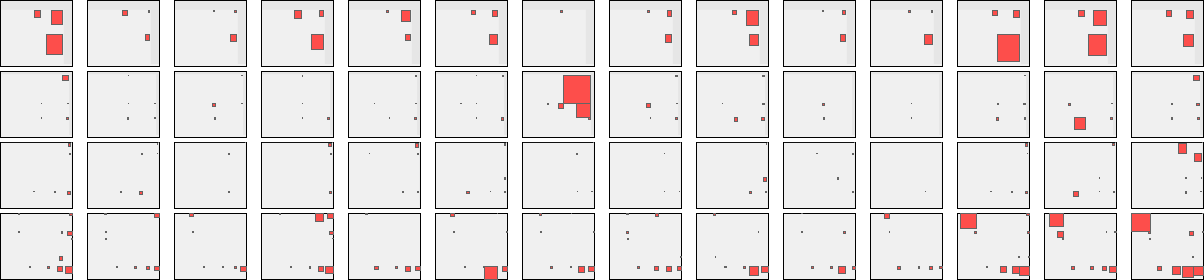
\includegraphics[width=17cm]{images/squaremap001.png}
%  \caption{Square, only changes, no log scale, global normalization}
%\end{figure*}

%\begin{figure*}[htb]
%  \centering
%  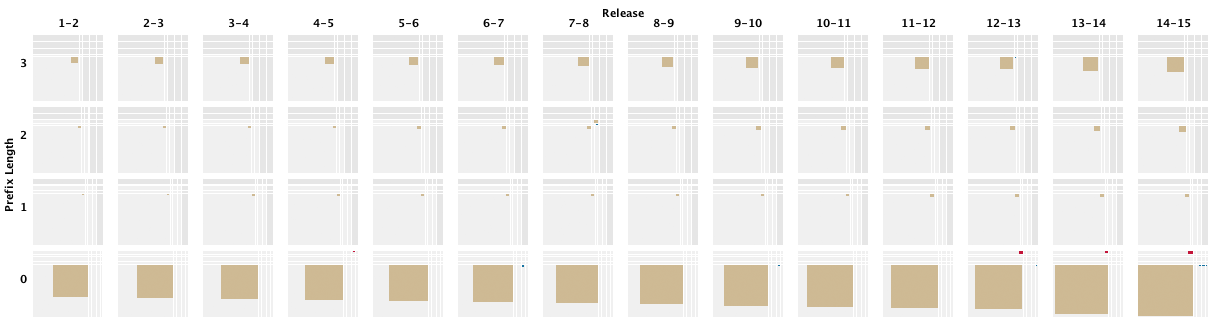
\includegraphics[width=17cm]{images/squaremap011.png}
%  \caption{Squaremap, only changes, log scale, global normalization}
%\end{figure*}

%\begin{figure}[htb]
%  \centering
%  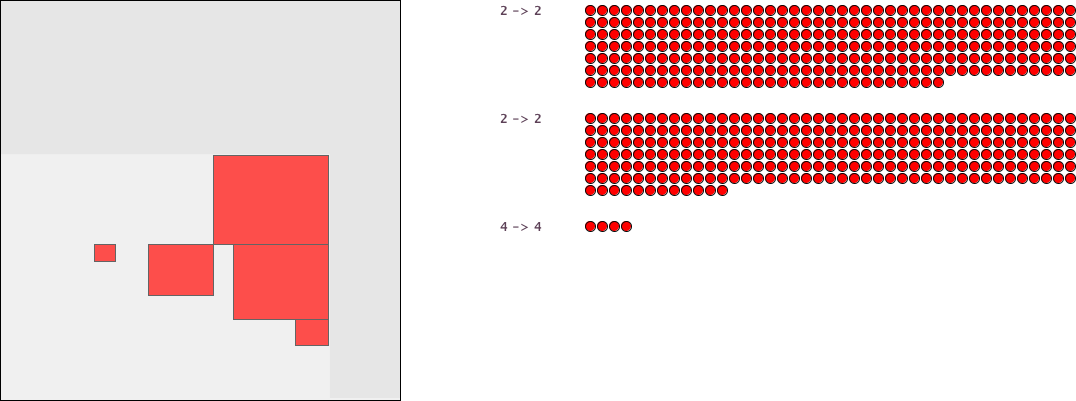
\includegraphics[width=8cm]{images/squaremap_detalhe.png}
%  \caption{}
%\end{figure}
